\section{Exploration and Analysis}
    \subsection{What makes a movie successful?}
        % We would like you to explore what makes a movie popular and/or successful.
        \paragraph{}
            In order to ascertain which factors are most influential in determining the
                success of a movie, it is necessary to first define what constitutes success.
            For the purpose of this analysis, success is defined as the movie's revenue.
            By examining the correlations between the movie's revenue and other factors, we
                can gain insight into which factors have the greatest impact on the success of
                a movie.
            These correlations are visualised in Figure \ref{fig-heatmap}.

            \begin{figure}[H]
                \centering
                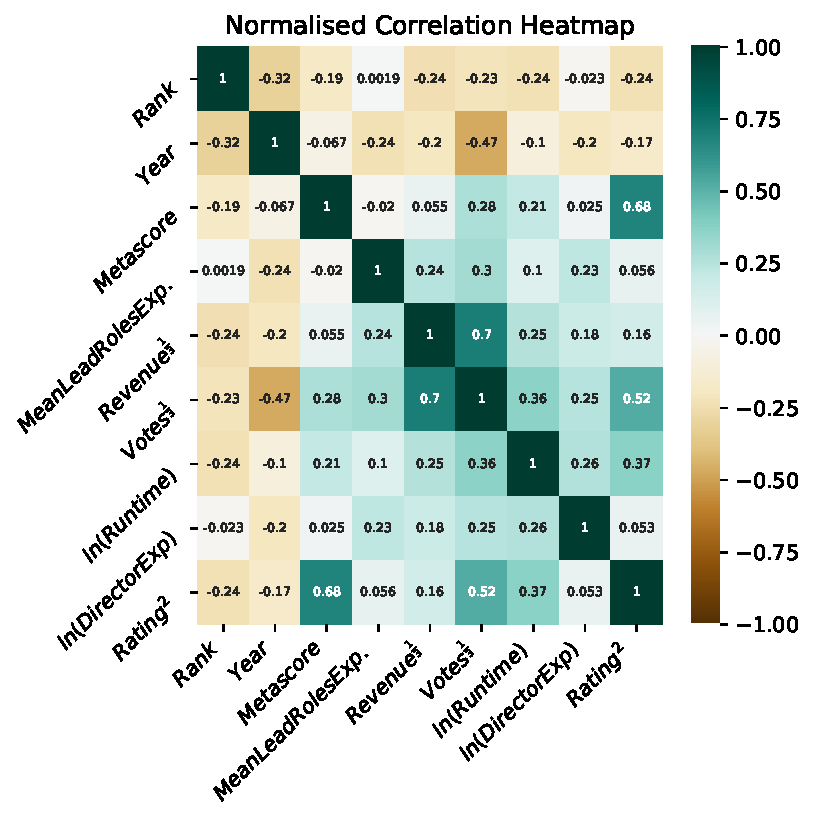
\includegraphics[width=0.8\linewidth]{Final/Normalised Correlation Heatmap.pdf}
                \caption[short]{
                    A heatmap illustrating the strength of correlations between various normalised
                    variables from the IMDb dataset \cite{data:IMDb}.
                    The Pearson's Product Moment Correlation Coefficient is used to calculate the
                        strength of the correlations.
                    These variables included Rank, Year, Metascore, Revenue, Votes, Runtime, and
                        Rating.
                    Additionally, two more variables were calculated from the TMD data
                        \cite{data:TMD}: MeanLeadRolesExperience and DirectorExperience.
                    Each correlation is represented by a value between -1 and 1, with weaker
                        correlations having values closer to 0, and negative correlations having
                        negative values and positive correlations having positive values.
                }\label{fig-heatmap}
            \end{figure}

        \paragraph{}
            Figure \ref{fig-heatmap} reveals a strong positive correlation (0.7) between a
                movie's revenue and the number of votes it receives on IMDb, suggesting that
                the more votes a movie receives, the higher its revenue is likely to be.
            Additionally, the heatmap shows moderate positive correlations between the
                movie's revenue and its runtime (0.25) and between the movie's revenue and the
                experience of the actors in lead roles (0.24), indicating that longer runtimes
                and more experienced actors may be associated with higher revenues.
            In contrast, there is a moderate negative correlation between a movie's revenue
                and its rank on IMDb (-0.24), suggesting that higher ranks on IMDb do not
                necessarily translate to higher revenues.
            These four correlations are shown in more detail in Figure
                \ref{fig-revenue-factors}.

            \begin{figure}[H]
                \centering
                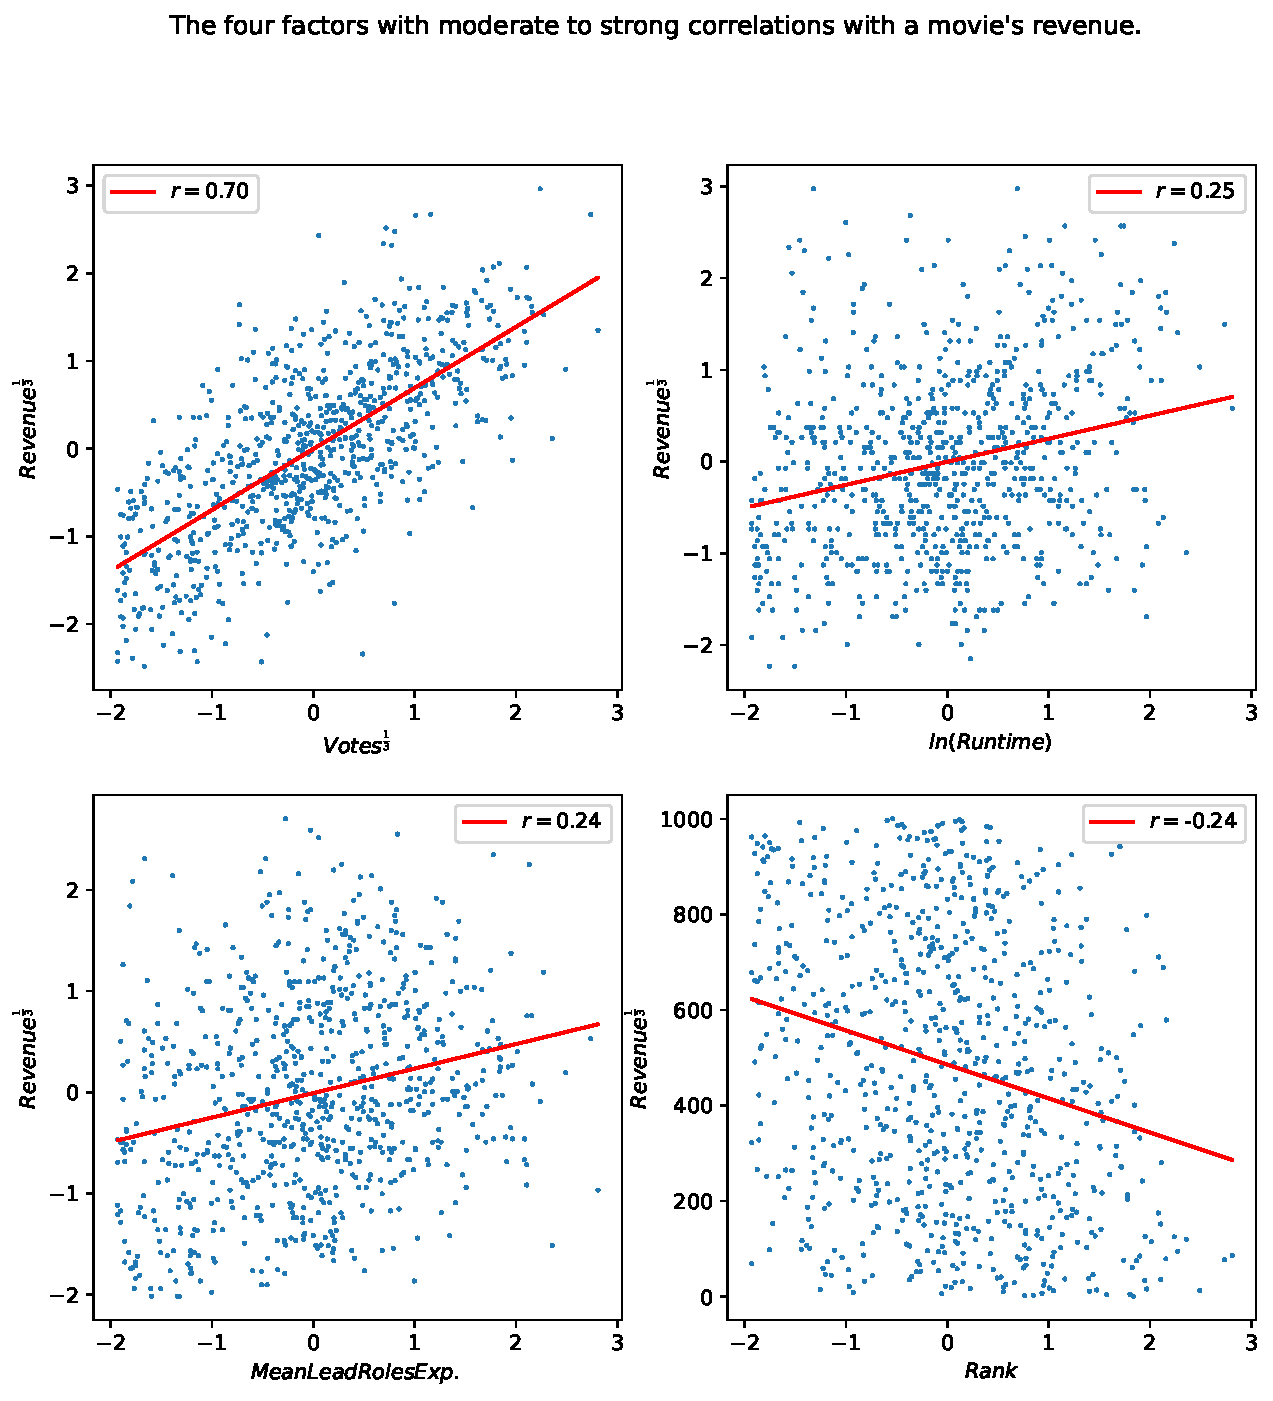
\includegraphics[width=0.8\linewidth]{Final/Revenue Factors.pdf}
                \caption[short]{
                    Scatter plots showing the relationships between a movie's revenue and the four
                    factors with moderate or strong correlations.
                }\label{fig-revenue-factors}
            \end{figure}

    \subsection{The relationship between a movie's ranked position and its number of votes}
        % We would also like you to visualise the distribution of ranked position and
        % number of votes, and comment on the relationship between them.
        \paragraph{}

    % Suggested 500 words for individual report; proportionately longer for group
    % projects).
    % Revenue Multiple Regression
    \subsection{What factors can predict box office success?}
    % We would like you to explore what makes a movie popular and/or successful.
        \paragraph{}
        In order to further analyze the correlations between the various movie details
        and the revenue they generated, we created a multiple regression model using the
        normalized data we collected. 
        The target variable was the normalised revenue, with the rest of the dataset as the 
            predictor variables, excluding Genre and Title.
        $Votes^\frac{1}{3}$ was excluded as it is causally linked to Revenue; the more votes, the more people bought movie tickets. 
        The model uses Ordinary Least Squares regression and a constant column has been added to show y-intercept.
        The summary results are provided in Table \ref{tab-revenue-ols-summary}.
        \begin{table}[H]
            \begin{center}
                \begin{tabular}{lclc}
                    \toprule
                    \textbf{Dep. Variable:}           &  $Revenue^{\frac{1}{3}}$   & \textbf{  R-squared:         } &     0.404   \\
                    \textbf{Model:}                   &       OLS        & \textbf{  Adj. R-squared:    } &     0.393   \\
                    \textbf{Method:}                  &  Least Squares   & \textbf{  F-statistic:       } &     36.60   \\
                    \textbf{No. Observations:}        &         826      & \textbf{  AIC:               } &     1921.   \\
                    \textbf{Df Residuals:}            &         810      & \textbf{  BIC:               } &     1996.   \\
                    \textbf{Df Model:}                &          15      & \textbf{  Prob (F-statistic):} &  1.35e-80   \\
                    \textbf{Covariance Type:}         &    nonrobust     & \textbf{  Log-Likelihood:    } &   -944.32   \\
                    \bottomrule
                \end{tabular}
                \begin{tabular}{lcccccc}
                                                    & \textbf{coef} & \textbf{std err} & \textbf{t} & \textbf{P$> |$t$|$} & \textbf{[0.025} & \textbf{0.975]}  \\
                    \midrule
                    \textbf{$const$}                &     114.0116  &       19.712     &     5.784  &         0.000        &       75.319    &      152.705     \\
                    \textbf{$Rank$}                 &      -0.0006  &        0.000     &    -5.654  &         0.000        &       -0.001    &       -0.000     \\
                    \textbf{$Year$}                 &      -0.0565  &        0.010     &    -5.770  &         0.000        &       -0.076    &       -0.037     \\
                    \textbf{$Metascore$}            &       0.0416  &        0.038     &     1.093  &         0.275        &       -0.033    &        0.116     \\
                    \textbf{$Mean Lead Roles Exp.$} &       0.1125  &        0.030     &     3.793  &         0.000        &        0.054    &        0.171     \\
                    \textbf{$ln(Runtime)$}          &       0.1705  &        0.033     &     5.203  &         0.000        &        0.106    &        0.235     \\
                    \textbf{$ln(Director Exp)$}     &       0.0507  &        0.029     &     1.756  &         0.079        &       -0.006    &        0.107     \\
                    \textbf{$Rating^2$}             &       0.0816  &        0.041     &     2.013  &         0.044        &        0.002    &        0.161     \\
                    \textbf{$Action$}               &       0.1824  &        0.070     &     2.598  &         0.010        &        0.045    &        0.320     \\
                    \textbf{$Adventure$}            &       0.4765  &        0.074     &     6.452  &         0.000        &        0.332    &        0.621     \\
                    \textbf{$Sci-Fi$}               &       0.0318  &        0.087     &     0.364  &         0.716        &       -0.140    &        0.203     \\
                    \textbf{$Thriller$}             &      -0.0395  &        0.078     &    -0.504  &         0.615        &       -0.193    &        0.114     \\
                    \textbf{$Comedy$}               &       0.1145  &        0.072     &     1.599  &         0.110        &       -0.026    &        0.255     \\
                    \textbf{$Drama$}                &      -0.5579  &        0.071     &    -7.877  &         0.000        &       -0.697    &       -0.419     \\
                    \textbf{$Romance$}              &      -0.0243  &        0.084     &    -0.288  &         0.773        &       -0.190    &        0.141     \\
                    \textbf{$Crime$}                &      -0.0545  &        0.082     &    -0.664  &         0.507        &       -0.216    &        0.107     \\
                    \bottomrule
                \end{tabular}
                \begin{tabular}{lclc}
                    \textbf{Omnibus:}       &  2.065 & \textbf{  Durbin-Watson:     } &    2.048  \\
                    \textbf{Prob(Omnibus):} &  0.356 & \textbf{  Jarque-Bera (JB):  } &    1.964  \\
                    \textbf{Skew:}          & -0.055 & \textbf{  Prob(JB):          } &    0.375  \\
                    \textbf{Kurtosis:}      &  2.788 & \textbf{  Cond. No.          } & 1.53e+06  \\
                \bottomrule
                \end{tabular}
            \end{center}
            
            \caption[short]{Multiple regression results with $Revenue^{\frac{1}{3}}$ as the dependent variable
                            and the normalised data as the independent variable. The OLS approach was used to
                            find the best fit. The residuals for this model are shown in fig \ref{fig-revenue-ols-residuals}}\label{tab-revenue-ols-summary}
        \end{table}
        This model performs respectably, explaining about  40\% of the variance in user ratings.
        It is also statistically significant, getting a very small  $P(F-statistic)$.
        This indicates that the revenue of a movie can be predicted from the data present in the dataset,
            albeit not extremely well.
        However, the relatively good $R^2$ value does indicate a well performing model, as such
            we can postulate that at least some of these factors are impactful on the revenue a 
            movie makes.
        There are also a few interesting observations that can be made about this data.

        % Director vs Actor for selling tickets
        One such observation is that the experience of lead actors has a statistically significant effect
            on movie ticket sales (p<0.05), while the experience of directors does not (p>0.05). 
        This raises the question of whether the director has as much of an impact as the actors when it
            comes to selling tickets.
        A possible explanation is the fact that promotional posters for movies often focus on the
            actors \cite{label}, with their faces being the first thing a consumer sees.
        Actors who have been in many movies tend to be more recognisable, making potential consumers more
            likely to see a movie they are in and thus improving ticket sales.
        In contrast, the director's name is usually the only thing featured on the poster, drawing little
            attention and thus being less impactful.
        This idea is inline with previous research \cite{label}.

        % Meta score vs Rating
        Another insight is that while critic scores are not reliable predictors of a
            film's revenue user ratings are, with p>0.05 and p<0.05 respectively.
        This raises the question of why there is a difference between these two forms of rating; they both correlate
            strongly with each other (see fig \ref{label}) so it is reasonable to assume they would have similar 
            strength as predictor variables.
        A possible explanation could be due to the relatively short time movies appear in box office for.
        With revenue only being calculated during this time, consumers would have more reliance on friends
            and family than a review that would be published a while after the movie came out.
        With this in mind, it is reasonable to say that critics do not appear to be able to predict the Likelihood
            of a movie becoming a blockbuster.
        
        % Genre notes
        Finally, there are some interesting notes about the impact of genre has on the box office success of a movie.
        Adventure seems to have the biggest positive impact on box office success, its coefficient is $\sim$ 0.48.
        Drama appears to have the largest negative impact on box office success, with a coefficient of $\sim$ -0.56.
    \subsection{What predicts movie success, are critics truly  makes a movie successful?}
        % We would like you to explore what makes a movie popular and/or successful.
        \paragraph{}
        % Success metric definition
        To analyze the effect critics had on predicting general success of a movie, a actual metric of movie success is
            needed.
        The metric we used was $Success = \frac{Revenue^\frac{1}{3} + Rating^2}{2}$.
        The reasoning behind this is quite simple, Revenue and Rating can both be used as metrics of movie success,
            and Figure \ref{fig-heatmap} shows that they are not strongly correlated, meaning they describe independent
            aspects of success. 
        Therefore, the mean of both will provide a more comprehensive measure of the end success of a movie.
        We will refer to this metric as success from now on.
        
        To investigate the ability for critics to predict movie success, we present a multiple regression model,
            with the target variable being the success metric. 
        We used the rest of the normalised dataset for predictor variables, excluding the $Revenue^\frac{1}{3}$, $Rating^2$,
            Genre and Title columns.
        Genre and Title were excluded as they are not quantative data and $Revenue^\frac{1}{3}$ and $Rating^2$ were excluded
            as they are causally  linked to the success metric.
        We use the same approach as in Table \ref{tab-revenue-ols-summary}, with a constant column and using OLS.
        The summary results are provided in Table \ref{tab-success-ols-summary}.
        \begin{table}[h]
            \begin{center}
                \begin{tabular}{lclc}
                    \toprule
                    \textbf{Dep. Variable:}           &     Success      & \textbf{  R-squared:         } &     0.758   \\
                    \textbf{Model:}                   &       OLS        & \textbf{  Adj. R-squared:    } &     0.753   \\
                    \textbf{Method:}                  &  Least Squares   & \textbf{  F-statistic:       } &     169.1   \\
                    \textbf{Date:}                    & Fri, 31 Mar 2023 & \textbf{  Prob (F-statistic):} & 2.67e-237   \\
                    \textbf{Time:}                    &     15:35:16     & \textbf{  Log-Likelihood:    } &   -342.78   \\
                    \textbf{No. Observations:}        &         826      & \textbf{  AIC:               } &     717.6   \\
                    \textbf{Df Residuals:}            &         810      & \textbf{  BIC:               } &     793.0   \\
                    \textbf{Df Model:}                &          15      & \textbf{                     } &             \\
                    \textbf{Covariance Type:}         &    nonrobust     & \textbf{                     } &             \\
                    \bottomrule
                \end{tabular}
                \begin{tabular}{lcccccc}
                                                    & \textbf{coef} & \textbf{std err} & \textbf{t} & \textbf{P$> |$t$|$} & \textbf{[0.025} & \textbf{0.975]}  \\
                    \midrule
                    \textbf{$const$}                &     -49.4262  &       10.871     &    -4.547  &         0.000        &      -70.765    &      -28.087     \\
                    \textbf{$Rank$}                 &      -0.0001  &     5.42e-05     &    -2.173  &         0.030        &       -0.000    &    -1.14e-05     \\
                    \textbf{$Year$}                 &       0.0246  &        0.005     &     4.560  &         0.000        &        0.014    &        0.035     \\
                    \textbf{$Metascore$}            &       0.1858  &        0.015     &    12.006  &         0.000        &        0.155    &        0.216     \\
                    \textbf{$Mean Lead Roles Exp.$} &      -0.0003  &        0.015     &    -0.022  &         0.983        &       -0.029    &        0.028     \\
                    \textbf{$Votes^{\frac{1}{3}}$}  &       0.5669  &        0.020     &    28.674  &         0.000        &        0.528    &        0.606     \\
                    \textbf{$ln(Runtime)$}          &       0.0820  &        0.016     &     5.185  &         0.000        &        0.051    &        0.113     \\
                    \textbf{$ln(Director Exp)$}     &      -0.0318  &        0.014     &    -2.286  &         0.023        &       -0.059    &       -0.004     \\
                    \textbf{$Action$}               &      -0.0532  &        0.034     &    -1.561  &         0.119        &       -0.120    &        0.014     \\
                    \textbf{$Adventure$}            &       0.1279  &        0.036     &     3.554  &         0.000        &        0.057    &        0.199     \\
                    \textbf{$Sci-Fi$}               &      -0.2271  &        0.043     &    -5.300  &         0.000        &       -0.311    &       -0.143     \\
                    \textbf{$Thriller$}             &      -0.0610  &        0.038     &    -1.610  &         0.108        &       -0.135    &        0.013     \\
                    \textbf{$Comedy$}               &       0.0376  &        0.035     &     1.087  &         0.277        &       -0.030    &        0.106     \\
                    \textbf{$Drama$}                &      -0.0391  &        0.035     &    -1.133  &         0.258        &       -0.107    &        0.029     \\
                    \textbf{$Romance$}              &      -0.0858  &        0.041     &    -2.103  &         0.036        &       -0.166    &       -0.006     \\
                    \textbf{$Crime$}                &      -0.0795  &        0.040     &    -2.003  &         0.046        &       -0.157    &       -0.002     \\
                    \bottomrule
                \end{tabular}
                \begin{tabular}{lclc}
                    \textbf{Omnibus:}       &  4.789 & \textbf{  Durbin-Watson:     } &    1.882  \\
                    \textbf{Prob(Omnibus):} &  0.091 & \textbf{  Jarque-Bera (JB):  } &    5.907  \\
                    \textbf{Skew:}          & -0.021 & \textbf{  Prob(JB):          } &   0.0522  \\
                    \textbf{Kurtosis:}      &  3.412 & \textbf{  Cond. No.          } & 1.75e+06  \\
                    \bottomrule
                \end{tabular}
            \end{center}
        \caption[short]{Multiple Regression results summary}\label{tab-success-ols-summary}
    \end{table}

\begin{figure}[H]
    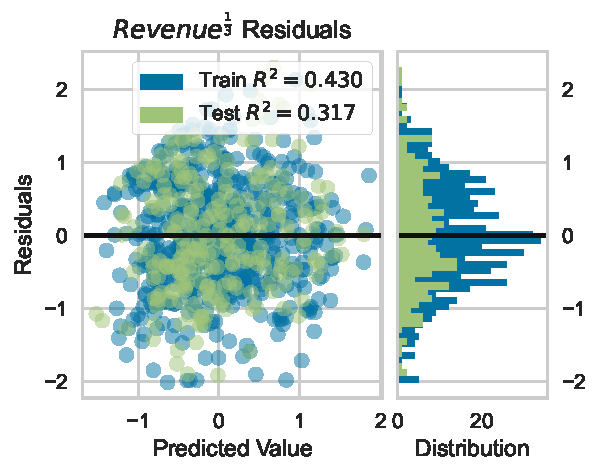
\includegraphics[width=\linewidth]{/Final/Revenue OLS Residuals.pdf}
    \caption[short]{title}\label{fig-revenue-ols-residuals}
\end{figure}
\newpage
asd
